\documentclass[11pt]{article}
  \usepackage{pslatex}
  \usepackage{amsmath}
  \usepackage{tikz}
  \advance\textwidth by2cm
  \advance\oddsidemargin by-1cm
  \advance\textheight by3cm
  \headheight 0pt\headsep 0pt

\begin{document}
  \thispagestyle{empty}

\begin{center}
  \Large\sf Advanced Algorithms, Fall 2012\\

  \medskip
  \large\sf Prof. Bernard Moret\\

  \medskip\bigskip
  \Large\bf Homework Assignment \#3\\

  \smallskip
  \normalsize\rm due Sunday night, Oct.\ 14
\end{center}

\bigskip\rm\noindent
\textit{Write your solutions in LaTeX using the template provided on the
Moodle and web sites and upload your PDF file through Moodle by 4:00 am
Monday morning, Oct.\ 15.}

\medskip\bigskip\rm\noindent
\emph{Question 1.}
Recall that the \emph{rank} of a node $v$, denoted as $r(v)$,
is defined as $\log w(v)$, where $w(v)$ is the number of nodes in the subtree rooted at $v$.
In the splay trees, we define its potential function as $\sum_{v} r(v)$.
Prove that among all possible binary trees of $n$ nodes,
the linked list has the maximum potential
and the complete binary tree has the minimum potential.

\noindent
{\bf Solution:}
We prove that a linked list has the maximum potential by contradiction using a ``prune and regraft'' technique.
Suppose a tree that is not a linked list has the maximum potential.
We arbitrarily choose a node $v$ such that both of its two children pointers are not \verb%nil%
(we can always find such kind of node $v$; otherwise, this tree will be a linked list),
then we prune off the left subtree of $v$ and regraft it to a leaf, say $l$, in the right subtree of $v$.
Clearly, the nodes on the path from $l$~(including $l$) to $v$~(excluding $v$) have rank increased
while other nodes' rank keep the same.
Thus, the potential of the new tree will increase,
which contradicts with the assumption that the initial tree has the maximum potential.

We prove that a complete binary tree~(CBT) has the maximum potential by contradiction.
Suppose a tree that is not a CBT has the maximum potential,
then we can find a node $v$ in it such that the subtree rooted at $v$ is not CBT, but both the two subtrees of $v$, $L_v$ and $R_v$, are CBTs; otherwise this tree will be a CBT.

\begin{figure}[!htp]
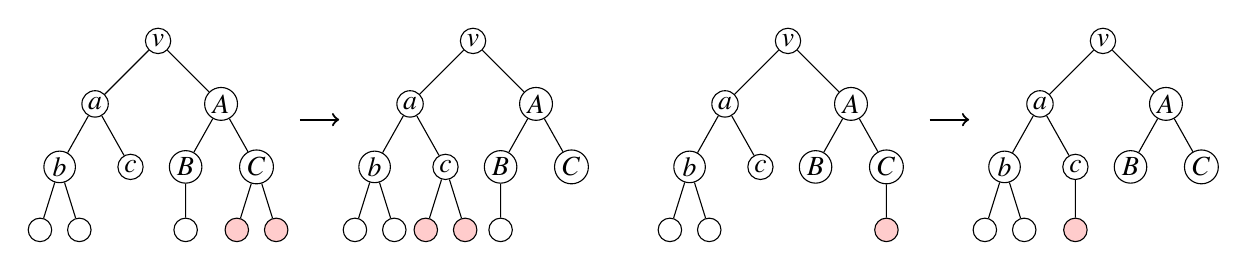
\begin{tikzpicture}
[level distance=8mm,
%, inner sep=1pt
every node/.style={draw, circle, inner sep=1pt},
level 1/.style={sibling distance=16mm},
level 2/.style={sibling distance=9mm},
level 3/.style={sibling distance=5mm, nodes={inner sep=3pt}}]

\begin{scope}
\node {$v$}
child {node{$a$}
    child{node{$b$}
     child{node{}} child{node{}}
    }
    child{node{$c$} }
}
child {node{$A$}
    child{node{$B$}
     child{node{}}
    }
    child{node{$C$}
     child{node[fill=red!20]{}} child{node[fill=red!20]{}}
    }
};
\end{scope}
\draw[->, thick] (1.8,-1) -- (2.3,-1);

\begin{scope}[xshift=4cm]
\node {$v$}
child {node{$a$}
    child{node{$b$}
     child{node{}} child{node{}}
    }
    child{node{$c$}
     child{node[fill=red!20]{}} child{node[fill=red!20]{}}
    }
}
child {node{$A$}
    child{node{$B$}
     child{node{}}
    }
    child{node{$C$}
    }
};
\end{scope}

\begin{scope}[xshift=8cm]
\node {$v$}
child {node{$a$}
    child{node{$b$}
     child{node{}} child{node{}}
    }
    child{node{$c$} }
}
child {node{$A$}
    child{node{$B$}
    }
    child{node{$C$}
     child{node[fill=red!20]{}}
    }
};
\end{scope}
\draw[->, thick] (9.8,-1) -- (10.3,-1);
\begin{scope}[xshift=12cm]
\node {$v$}
child {node{$a$}
    child{node{$b$}
     child{node{}} child{node{}}
    }
    child{node{$c$}
     child{node[fill=red!20]{}}
    }
}
child {node{$A$}
    child{node{$B$}
    }
    child{node{$C$}
    }
};
\end{scope}
\end{tikzpicture}

\caption{
%$L_v$ and $R_v$ has the same height.
First two subfigures: move the 2 red nodes of $R_v$ to the corresponding positions in $L_v$,
and the last layer of $L_v$ becomes full.
Last two subfigures: move the 1 red node of $R_v$ to the corresponding position in $L_v$,
and the last layer of $R_v$ becomes empty.}
\label{fig1}
\end{figure}


First consider the case that $L_v$ and $R_v$ have the same height.
Notice that the last layer of $L_v$ or $R_v$ is not full;
otherwise the subtree rooted at $v$ will be a CBT.
We rotate $R_v$ to make its nodes in the last layer in the right side.
Now we try to move as many nodes in the last layer of $R_v$ as possible to the corresponding 
empty positions of $L_v$.
If there are enough nodes in the last layer of $R_v$, then the last layer of $L_v$ will become full~(see the first 2 subfigures in figure~\ref{fig1});
otherwise, the last layer of $R_v$ will become empty~(see the last 2 subfigures in figure~\ref{fig1}).
Consider a pair of corresponding nodes, for example, $a$ and $A$.
Clearly, the changes of the weight of $a$ and $A$ are summed to 0, i.e., 
$w'(a) = w(a) + \delta$ and $w'(A) = w(A) - \delta$,
where $w'(a)$ and $w'(A)$ is the weight of node $a$ and $A$ after the movement respectively.
Consider the potential change in the case that the last layer of $L_v$ becomes full after movement~(the first 2 subfigures in figure~\ref{fig1}).
The potential increase of node $a$ is 
$$\Delta\Phi_{+} = \log(w'(a)) - \log(w(a)) = \log\left(\frac{w'(a) }{w'(a) - \delta}\right),$$
and the potential decrease of node $A$ is 
$$\Delta\Phi_{-} = \log(w(A)) - \log(w'(A)) = \log\left(\frac{w(A) }{w'(A) - \delta}\right).$$
Since before the movement the last layer of $R_v$ is not full while after movement $L_v$ becomes full,
we have $w'(a) > w(A)$, which means $\Delta\Phi_{+} < \Delta\Phi_{-}$.
Thus, the potential change for $a$ and $A$ is $\Delta\Phi = \Delta\Phi_{+} - \Delta\Phi_{-} < 0$.
The same argument can be posed on other pairs. 
The only difference is that the potential change might be equal to zero 
if the chosen two pairs is not the roots of $L_v$ and $R_v$,
since the last layer in a subtree might be full before movement.
For example, the potential change for $c$ and $C$ is 0.
Combining the potential change of all pairs of nodes, 
we obtain that the potential for the whole subtree rooted at $v$ decreases after movement.
For the case that the last layer of $R_v$ becomes empty after movement~(the last two subfigures in figure~\ref{fig1}), we have 
$$\Delta\Phi_{+} = \log(w'(a)) - \log(w(a)) = \log\left(\frac{w(a) + \delta}{w(a)}\right),$$
and
$$\Delta\Phi_{-} = \log(w(A)) - \log(w'(A)) = \log\left(\frac{w'(A) + \delta}{w'(A)}\right).$$
Now after movement, the last layer of $R_v$ becomes empty,
thus we have $w(a) > w'(A)$, which still implies $\Delta\Phi = \Delta\Phi_{+} - \Delta\Phi_{-} < 0$. 
Summarily, if $L_v$ and $R_v$ have the same height, we can perform a ``movement'' operation to reduce the potential.


\begin{figure}[!htp]
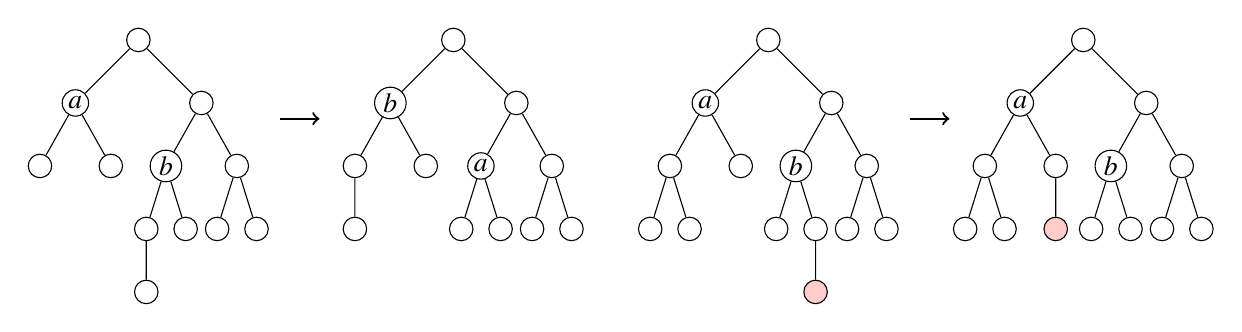
\begin{tikzpicture}
[level distance=8mm,
%, inner sep=1pt
every node/.style={draw, circle, inner sep=3pt},
level 1/.style={sibling distance=16mm, nodes={inner sep=3pt}},
level 2/.style={sibling distance=9mm, nodes={inner sep=3pt}},
level 3/.style={sibling distance=5mm, nodes={inner sep=3pt}},
level 4/.style={sibling distance=5mm, nodes={inner sep=3pt}}]

\begin{scope}
\node {}
child {node[inner sep=1pt]{$a$}
    child{node{}}
    child{node{}}
}
child {node{}
    child{node[inner sep=1pt]{$b$}
     child{node{}
      child{node{}}
     } 
     child{node{}}
    }
    child{node{}
     child{node{}} child{node{}}
    }
};
\end{scope}
\draw[->, thick] (1.8,-1) -- (2.3,-1);

\begin{scope}[xshift=4cm]
\node {}
    child{node[inner sep=1pt]{$b$}
     child{node{}
      child{node{}}
     }
     child{node{}}
    }
child {node{}
child {node[inner sep=1pt]{$a$}
    child{node{}}
    child{node{}}
}
    child{node{}
     child{node{}} child{node{}}
    }
};
\end{scope}

\begin{scope}[xshift=8cm]
\node {}
child {node[inner sep=1pt]{$a$}
    child{node{}
     child{node{}}
     child{node{}}
    }
    child{node{}}
}
child {node{}
    child{node[inner sep=1pt]{$b$}
     child{node{}
     }
     child{node{}
      child{node[fill=red!20]{}}
     }
    }
    child{node{}
     child{node{}} child{node{}}
    }
};
\end{scope}
\draw[->, thick] (9.8,-1) -- (10.3,-1);
\begin{scope}[xshift=12cm]
\node {}
child {node[inner sep=1pt]{$a$}
    child{node{}
     child{node{}}
     child{node{}}
    }
    child{node{}
     child{node[fill=red!20]{}}
    }
}
child {node{}
    child{node[inner sep=1pt]{$b$}
     child{node{}
     }
     child{node{}}
    }
    child{node{}
     child{node{}} child{node{}}
    }
};
\end{scope}
\end{tikzpicture}
\caption{
First two subfigures: if the last layer of $L_v$ is full, then we can find 
a subtree of the root of $R_v$~(subtree rooted at $b$ in the figure) that is bigger than $L_v$~(subtree rooted at $a$ in the figure) 
and we can exchange this subtree with $L_v$ to reduce the potential.
Last two subfigures: if neither of the last layer of $L_v$ or $R_v$ is full,
then we can find a subtree in $R_v$ that has the same height with $L_v$~(subtree rooted at $b$).
We can do the ``movement'' operation on $L_v$ and this subtree to reduce the potential.}
\label{fig2}
\end{figure}

Now consider the case that $L_v$ and $R_v$ do not have the same height.
Without loss of generality, suppose that $L_v$ is lower than $R_v$.
If the last layer of $L_v$ is full, then 
at least one of the two subtrees of the root of $R_v$ will be 
bigger than $L_v$~(see the first 2 subfigures of figure~\ref{fig2}).
We can exchange $L_v$ with this subtree and the rank of the root of $R_v$ decreases while other nodes' rank keep unchanged.
Thus, the potential of the subtree rooted at $v$ decreases.
The same argument can be posed on the case that the last layer of $R_v$ is full.
If neither is full, we can find a subtree $T$ in $R_v$ such that $T$ has the same height with $L_v$ and
the last layer of $T$ is not full. Then we apply the ``movement'' operation on $L_v$ and $T$ as shown in the first case.
Clearly, the potential will decrease, since the rank of the nodes on the path from the root of $T$ to the root of $R_v$ will decrease, and the potential restricted on $L_v$ and $T$ will also decrease, as we already have shown.

\bigskip\rm\noindent
\emph{Question 2.}
You are given a list of $n$ distinct items and a request sequence of accesses.
%You are given a list of $n$ distinct items. Let $f_i$ be the frequency of accessing item i, $f_i \ge 0$.
Find an offline static ordering of those $n$ items to minimize the total access cost and prove the optimality.

\noindent
{\bf Solution:}
Intuitively, these items should be arranged according to their accessing frequency.
Suppose the request frequency of the $i$-th item is $f_i$, $i=1,2,\cdots, n$.
Sort $f_1, f_2, \cdots, f_n$ in non-increasing order,
i.e., $f_{p_1} \ge f_{p_2} \ge \cdots \ge f_{p_n}$;
put the $p_k$-th symbol at the $k$-th position.\\
The optimality is guaranteed by the so-called \emph{rearrangement inequality},
which claims that for every choice of real numbers
$x_1\le x_2 \le \cdots \le x_n$ and $y_1\le y_2 \le \cdots \le y_n$,
we have $x_ny_1 + x_{n-1}y_2 + \cdots + x_1y_n \le
x_{\sigma_1} y_1 + x_{\sigma_2} y_2 + \cdots + x_{\sigma_n} y_n  \le
x_1y_1 + x_2y_2 + \cdots + x_ny_n$, where $\sigma$ can be any permutation of $\{1,\cdots,n\}$.
In other words, the reverse-order multiplication is the minimum.
In our problem, we are looking for a permutation $\sigma$~($\sigma_i$ is the index of the symbol that will be
arranged on the $i$-th position)
to minimize the total cost of $\sum_{k=1}^n k\cdot f_{\sigma_k}$.
We have $f_{p_1} \ge f_{p_2} \ge \cdots \ge f_{p_n}$
and $1 < 2 < \cdots < n$,
which means $\sigma_k=p_k$ is the permutation that has the minimum cost.


\medskip\bigskip\rm\noindent
\emph{Question 3.}
Show that the competitive analysis for the move-to-front algorithm against the static optimal algorithm is asymptotically tight.
(Hint: You need to give a general instance for which the cost of the move-to-front algorithm is twice as that of the static optimal algorithm in the limit.)

\noindent
{\bf Solution:}
Consider a list of $n$ items, $(1, 2, \cdots, n)$,
and $kn$ queries, which repeats $(n,n-1,n-2,\cdots,1)$ by $k$ times.
For move-to-front algorithm, clearly it costs $n$ for each query,
and the total cost for it is $kn^2$.
For the offline algorithm,
the symbols will be sorted as $(n, n-1, \cdots, 1)$,
and the total cost is $k \sum_{i=1}^n i = kn(n+1)/2$.
Thus, the competitive ratio is $2n/(n + 1)$, which is asymptotically 2.

\medskip\bigskip\rm\noindent
\emph{Question 4.}
You are given an array of $n$ items with distinct values (e.g.
non-negative integers) and you would like to pick up the
most valuable item. You can check the array only once by scanning from
the beginning to the end. When you
check the value of the i-th item during the scanning, you have to
decide whether to pick it up or not
immediately based on your experience (e.g. based on the values of all
previous items that you have checked).
If you pick it up, then it is your final choice and you cannot pick up
other item;
if you do not pick it up, then this item cannot be picked up in the
following process. All the $n!$
permutations are equally distributed. You are asked to design an
deterministic algorithm that it returns the most valuable item with
the probability strictly greater than $1/4$.

\noindent
{\bf Solution:}
This problem is a simplified version
of \emph{Secretary Problem}.
When the threshold is set as $n/e$~(not $n/2$),
we can prove that the probability of picking the most valuable item is $1/e$, which is optimal.\\
For our problem, the algorithm can be designed as follows.
Store the largest integer of the first half of the array in the scanning process.
When scanning the second half of the array,
compare the current integer with the largest integer of the first half and pick
it up if the current one is bigger.\\
Now we show that the probability that this algorithm returns the largest integer is strictly greater than $0.25$.
Consider the event that the largest integer is in the second half and the second largest integer is in the first half.
Clearly, for all permutations covered by this event our algorithm will returns the largest integer.
The probability for this event is $0.25$, since with probability $0.5$ the largest integer
is in the second half and with the same probability the second largest integer is in the first half.
Besides, if the third largest integer is in the first half,
the largest integer is in the second half and the second largest one is behind it,
our algorithm will also return the largest integer.
This probability of this event is larger than 0.
Thus, the probability that our algorithm returns the largest integer is strictly greater than $0.25$.



\end{document}






